\documentclass[../../main.tex]{subfiles}

\begin{document}

En este apartado se comenta sobre la implementación de la aplicación web realizada en \gls{shiny}.  \\

La aplicación se estructura para ofrecer dos finalidades:

\begin{itemize}
    \item La extracción de datos mediante la aplicación y visualización de los datos obtenidos
    \begin{figure}[H]
    \centering
    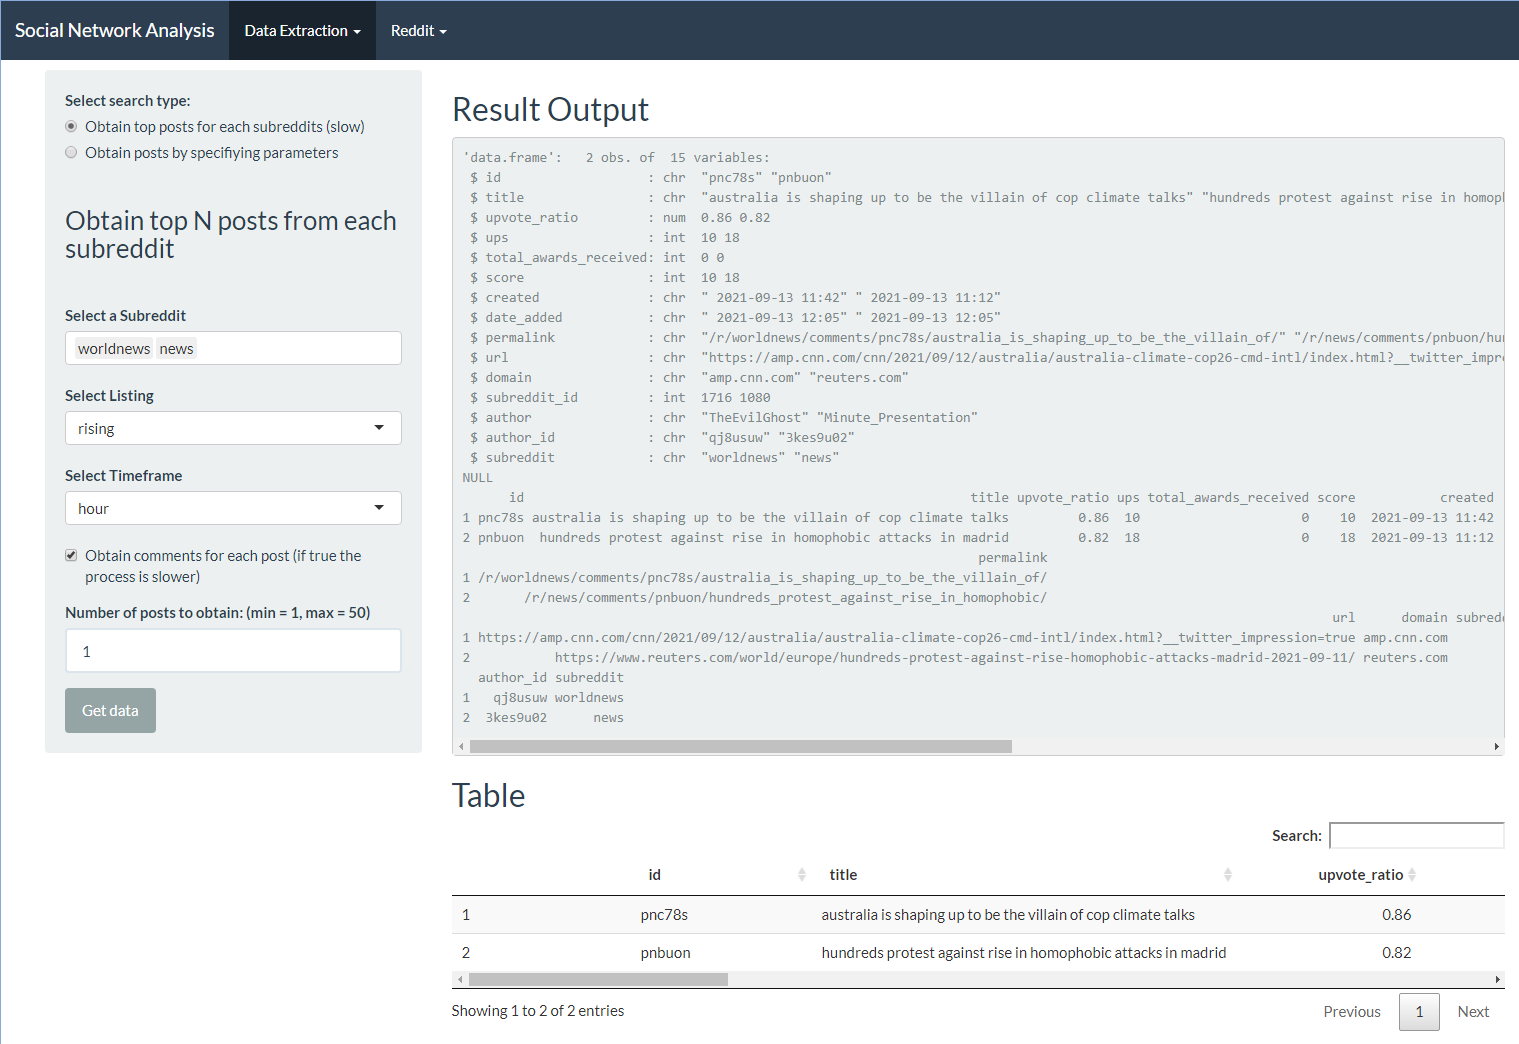
\includegraphics[width=400pt]{images/implementacion/app-extraction.png}
    \caption{Aplicación \Gls{shiny} - Extracción datos}
    \end{figure}
    \item La obtención de los datos del servidor de base de datos, visualizar estos datos y la aplicación de diversas técnicas para extraer información de estos datos.
    \begin{figure}[H]
    \centering
    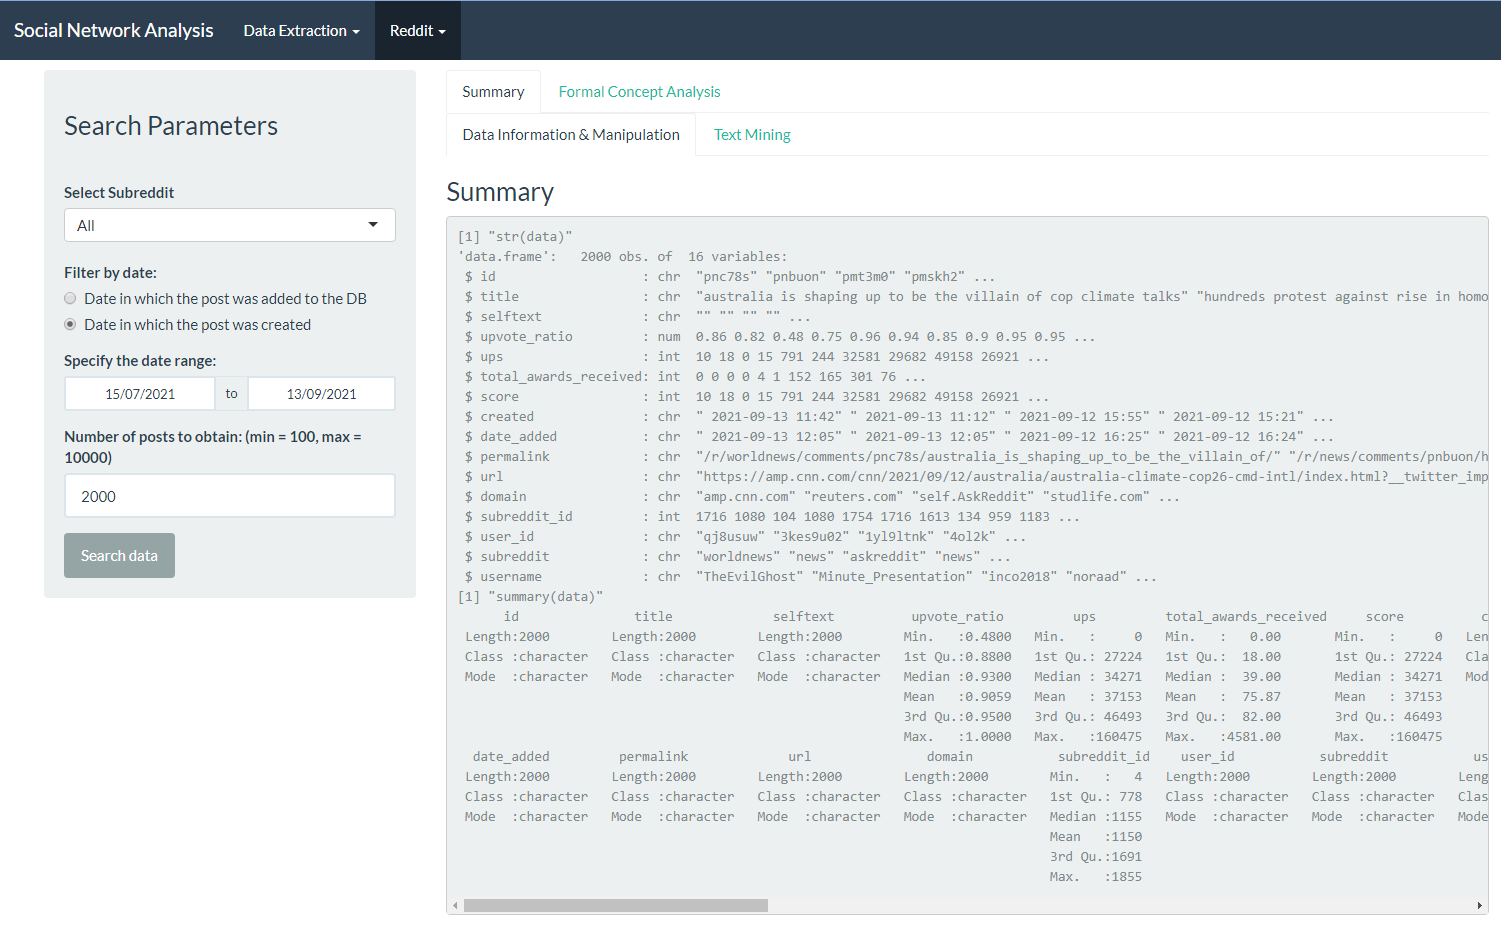
\includegraphics[width=400pt]{images/implementacion/app-reddit.png}
    \caption{Aplicación \Gls{shiny} - Análisis de los datos}
    \end{figure}
\end{itemize}

Para tener una aplicación web más modular y en la cual se intenta no repetir código, se han realizado las siguientes acciones:

\begin{itemize}
    \item Separar la lógica del apartado \gls{ui} y del apartado del servidor en dos ficheros diferentes, esto se realiza dado que contienen muchas líneas de código para una separación sobre la funcionalidad que realiza la misma.
    \item La implementación de módulos \gls{shiny} para los apartados \gls{ui} y de servidor, permitiendo reutilizar implementaciones ya existentes y tener una modularización de la aplicación más eficiente.
\end{itemize}

Esta implementación se encuentra distribuida en varios ficheros y carpetas, las cuales se mencionan a continuación:

\begin{itemize}
    \item \textbf{src/database/standard.R}. Fichero que implementa una entidad que conecta con el servidor de base de datos.
    \item \textbf{src/modules/server}. Carpeta que contiene los módulos diseñados para el apartado de servidor \Gls{shiny}
    \begin{itemize}
        \item \textbf{data.R}. Se encarga de ejecutar la lógica del apartado \textit{\Gls{reddit}} en cualquiera de sus opciones.
        \item \textbf{etl.R}. Se encarga de ejecutar la lógica del apartado \textit{Data Extraction}.
        \item \textbf{fca.R}. Se encarga de ejecutar todo el proceso de análisis del sub-apartado de \textit{Formal Concept Analysis}.
        \item \textbf{tm.R}. Se encarga de ejecutar la lógica del sub-apartado de \textit{Text Mining}.
    \end{itemize}
    \item \textbf{src/modules/ui}. Carpeta que contiene los módulos para el apartado gráfico del servidor \Gls{shiny}.
    \begin{itemize}
        \item \textbf{data.R}. Fichero que contiene la configuración de los elementos que se muestran en el apartado \textit{\Gls{reddit}} en cualquiera de sus opciones.
        \item \textbf{etl.R}. Fichero que contiene la configuración de los elementos que se muestran en el apartado \textit{Data Extraction}.
        \item \textbf{fca.R}. Fichero que contiene la configuración de los elementos que se muestran en el sub-apartado de \textit{Formal Concept Analysis}.
        \item \textbf{main.R}. Fichero en el cual se configura la plantilla general para toda la aplicación.
        \item \textbf{sidebar.R}. Fichero que contiene la configuración de los elementos de la barra lateral la cual se muestra de forma distinta según en el apartado.
    \end{itemize}
    \item \textbf{src/constants.R}. Fichero que contiene una serie de constantes necesarias para el funcionamiento de la aplicación.
    \item \textbf{src/functions.R}. Fichero que contiene una serie de funciones generales que son usadas en múltiples apartados de la aplicación.
    \item \textbf{src/includes.R}. Fichero que contiene la inclusión y compilación de todos los ficheros necesarios.
    \item \textbf{src/load.R}. Fichero que contiene la instalación y carga de todos los paquetes de R que son necesarios.
    \item \textbf{app.R}. Fichero que lanza la aplicación web.
    \item \textbf{globals.R}. Fichero que precarga una serie de datos y que es común a toda la aplicación web.
    \item \textbf{server.R}. Fichero que carga toda la lógica de la parte del servidor de la aplicación web.
    \item \textbf{ui.R}. Fichero que carga la parte gráfica de la aplicación web.
\end{itemize}

A continuación, se comenta los diferentes módulos usados en los apartados de la aplicación web.  \\

En este apartado se hace uso de los módulos de \gls{ui}: \textit{main, sidebar y etl}; Del lado del servidor se hace uso de los módulos: \textit{etl}.  \\
El fin de esta pantalla es disponer de la posibilidad de obtener información mediante la \gls{ipa} y visualizar los datos que se obtienen para una previsualización rápida.

\begin{figure}[H]
\centering
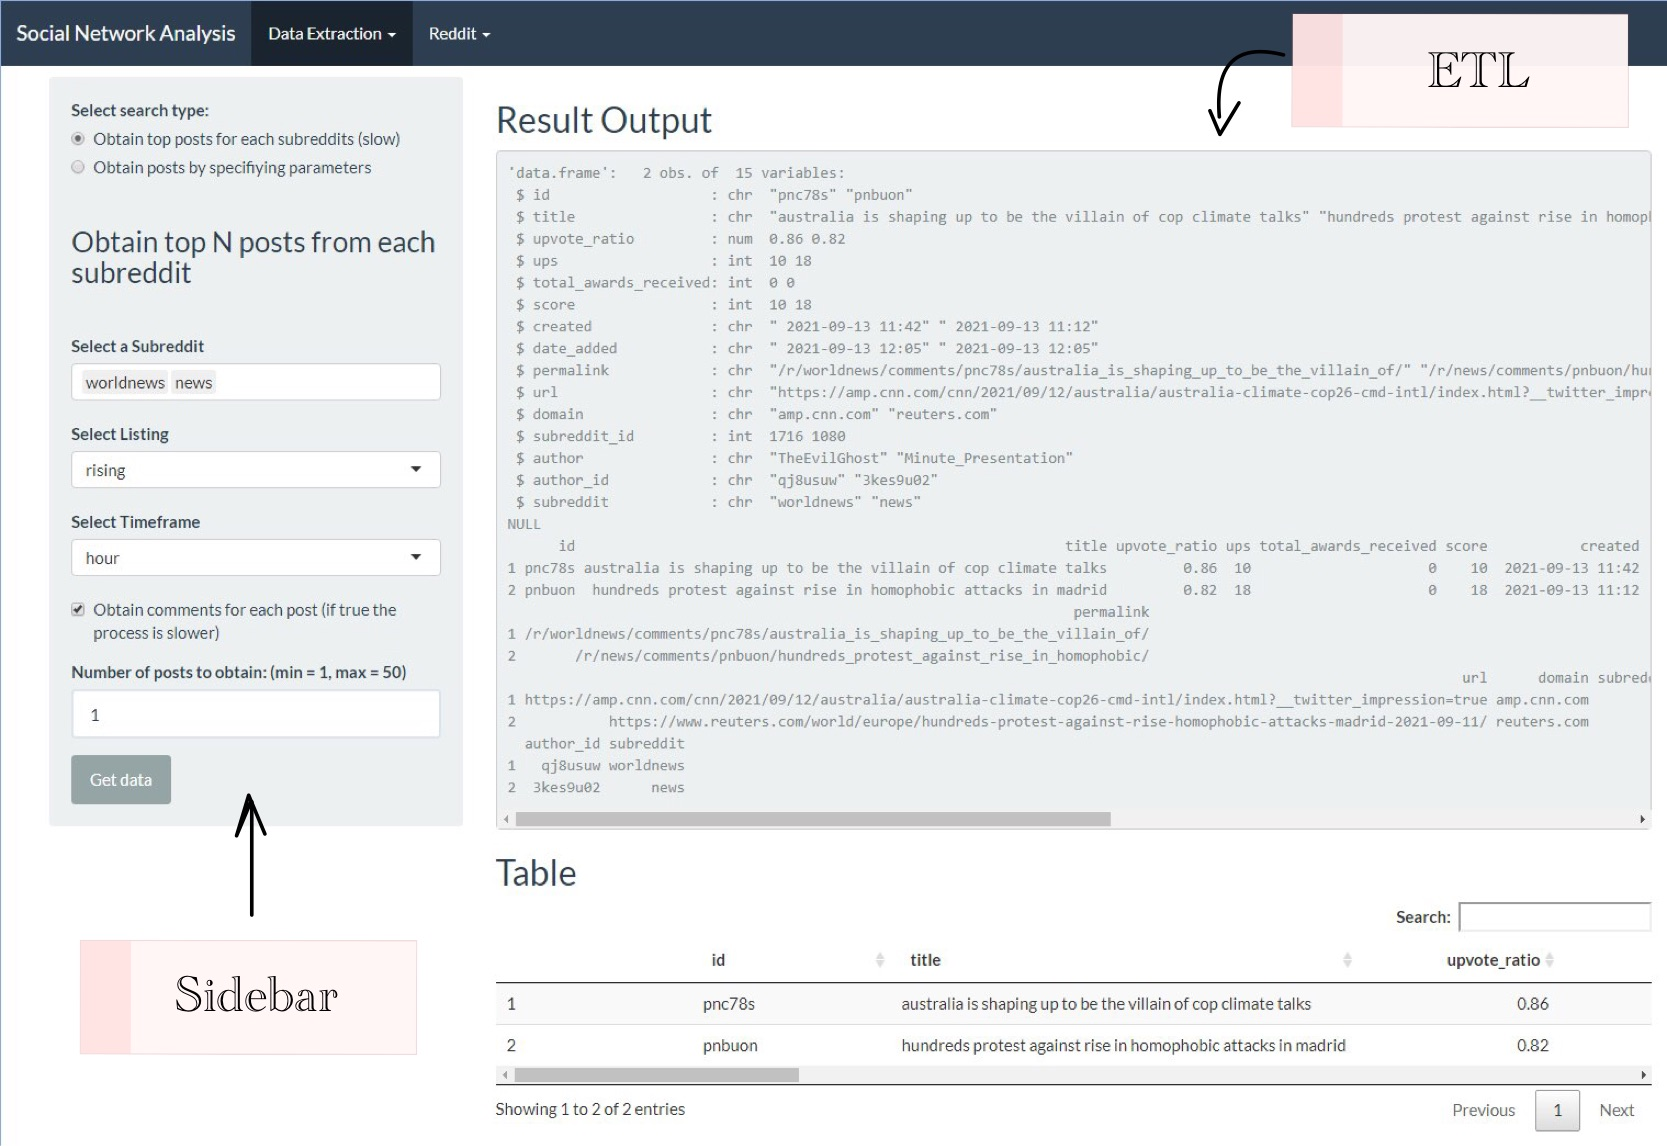
\includegraphics[width=400pt]{images/implementacion/app-1.jpg}
\caption{Aplicación \Gls{shiny} - Módulos en Extracción datos}
\end{figure}

En este apartado se hace uso de los módulos de \gls{ui}: \textit{main, sidebar y data}; Del lado del servidor se hace uso de los módulos: \textit{data}.  \\
El fin de esta pantalla es disponer de la posibilidad de obtener la información que se encuentra presente en el servidor de base de datos y realizar un tratamiento de los mismos para un estudio posterior del conjunto de datos obtenido.

\begin{figure}[H]
\centering
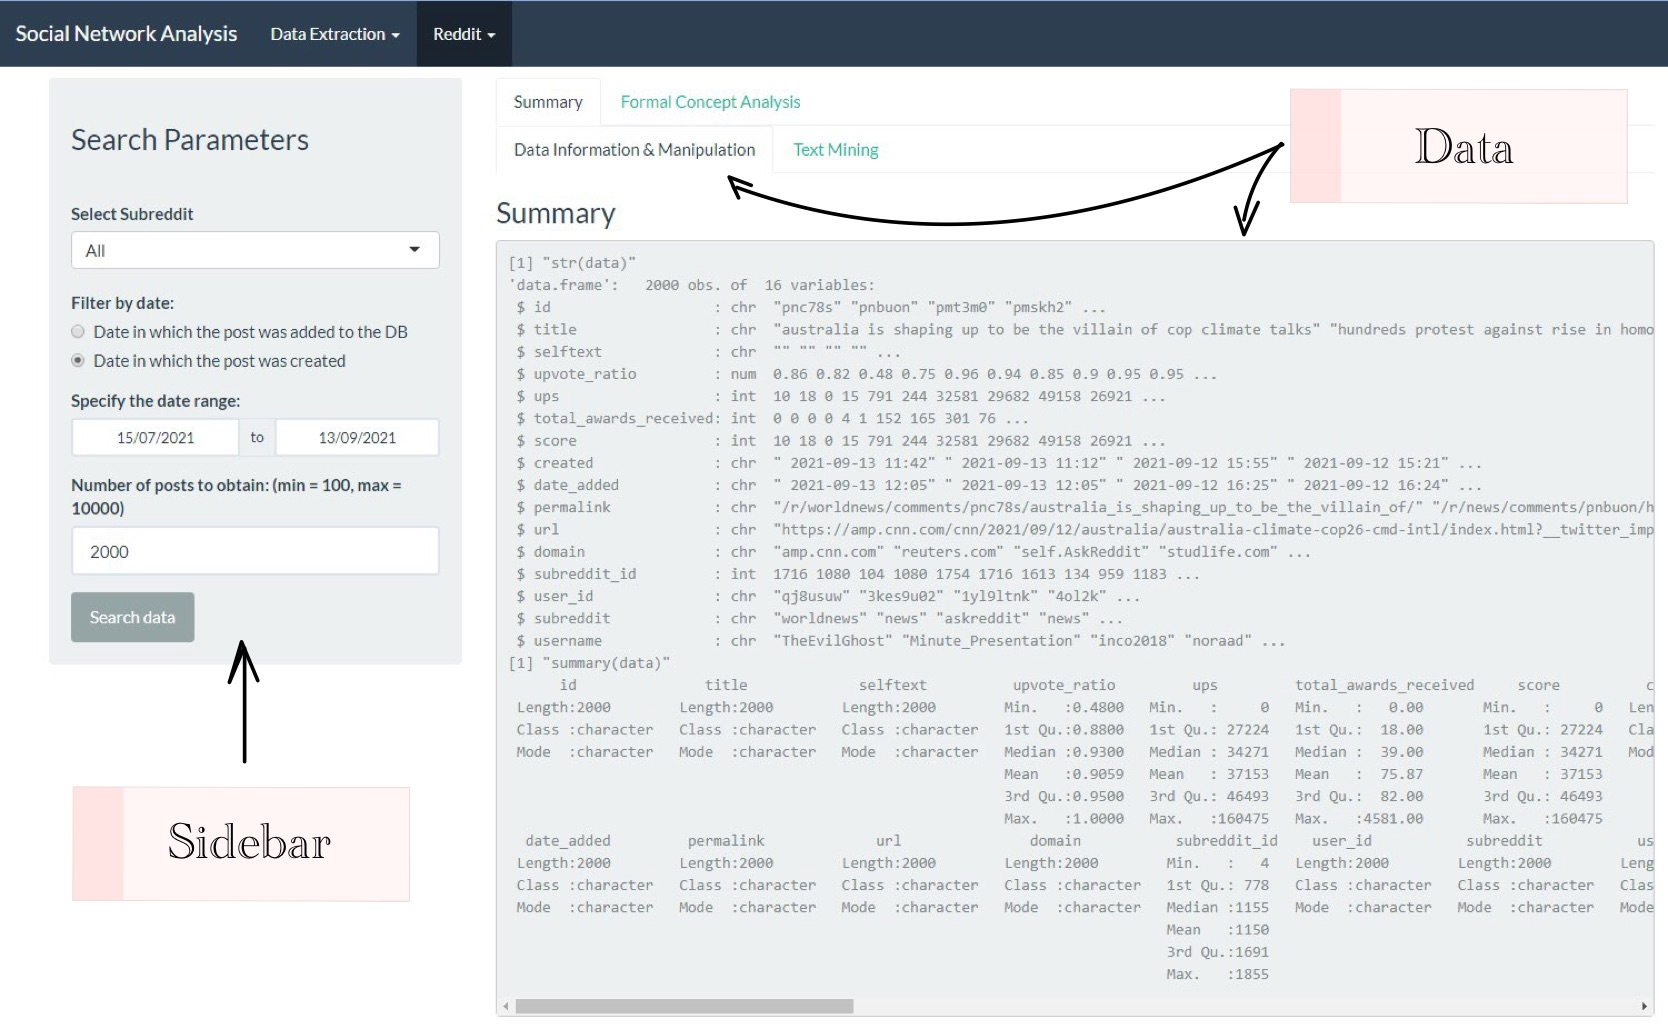
\includegraphics[width=400pt]{images/implementacion/app-2.jpg}
\caption{Aplicación \Gls{shiny} - Módulos en Visualización datos}
\end{figure}

En este apartado se hace uso de los módulos de \gls{ui}: \textit{main, sidebar y tm}; Del lado del servidor se hace uso de los módulos: \textit{tm}.  \\
El fin de esta pantalla es mostrar que información relevante se puede obtener de las publicaciones referente al texto presente en el título o descripción.

\begin{figure}[H]
\centering
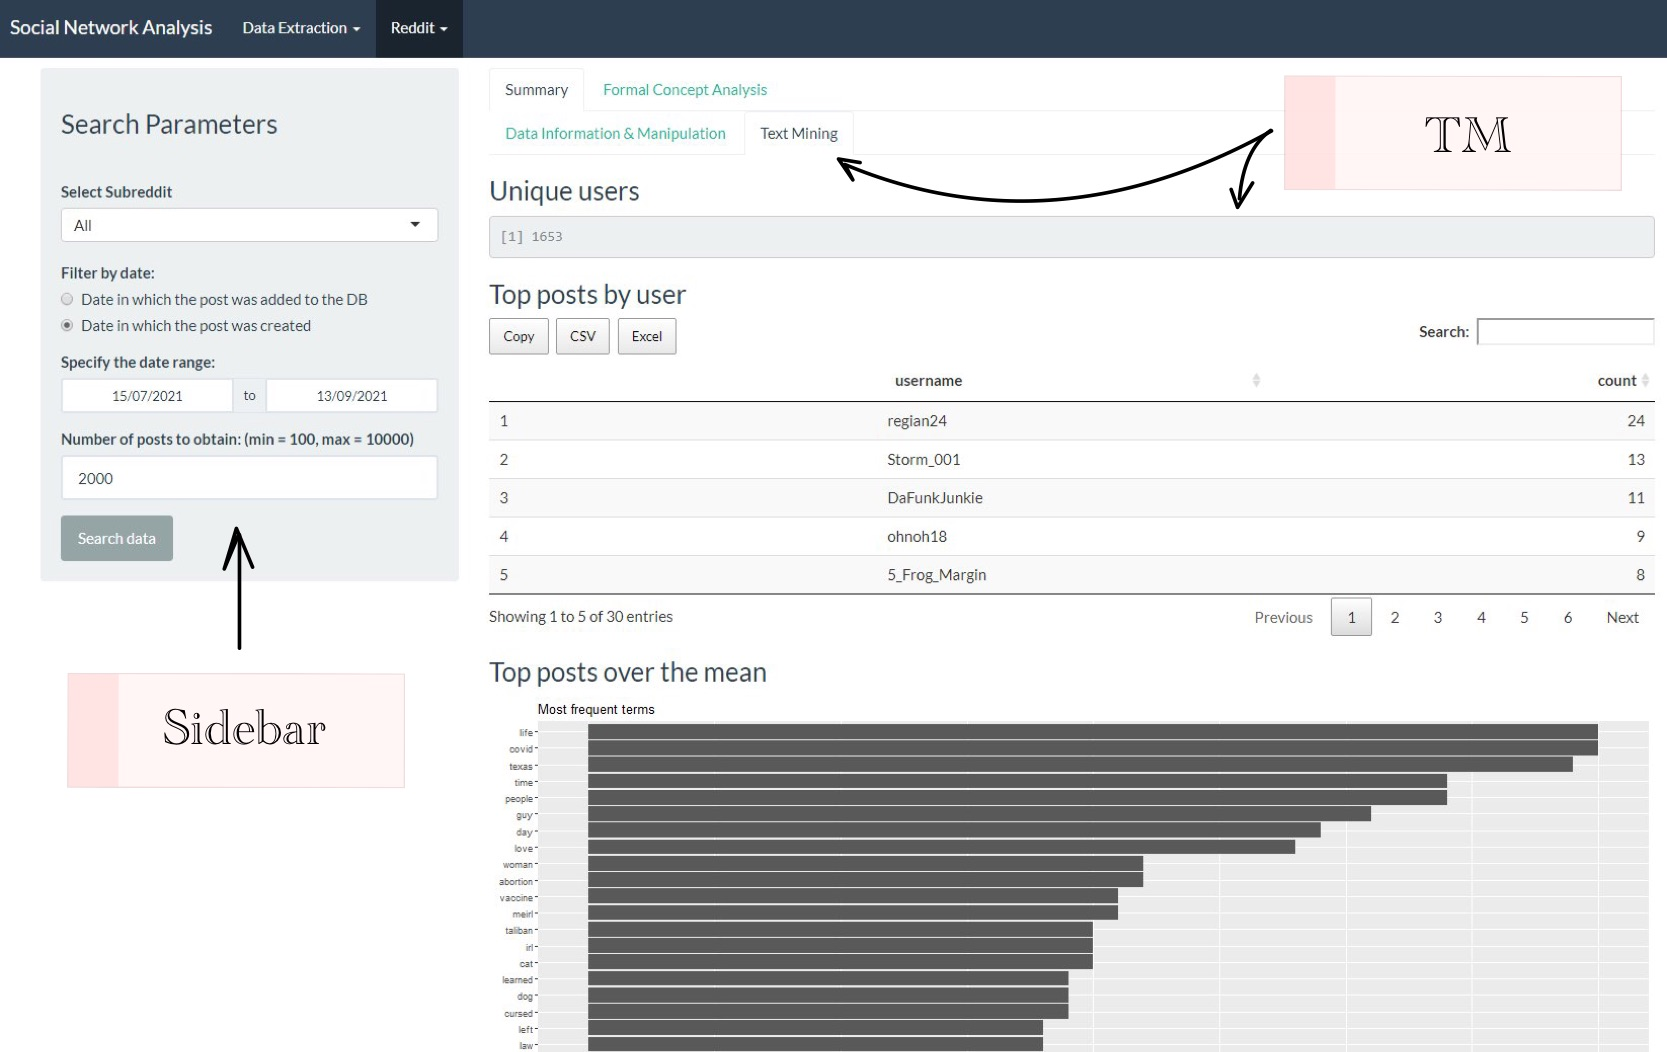
\includegraphics[width=400pt]{images/implementacion/app-3.jpg}
\caption{Aplicación \Gls{shiny} - Módulos en Minería de datos}
\end{figure}

En este apartado se hace uso de los módulos de \gls{ui}: \textit{main, sidebar y fca}; Del lado del servidor se hace uso de los módulos: \textit{fca}.  \\
El fin de esta pantalla es poder realizar un análisis del conjunto de datos en el cual se aplican diversas operaciones para poder ir extrayendo la información mediante el uso de \textit{\gls{afc}}.

\begin{figure}[H]
\centering
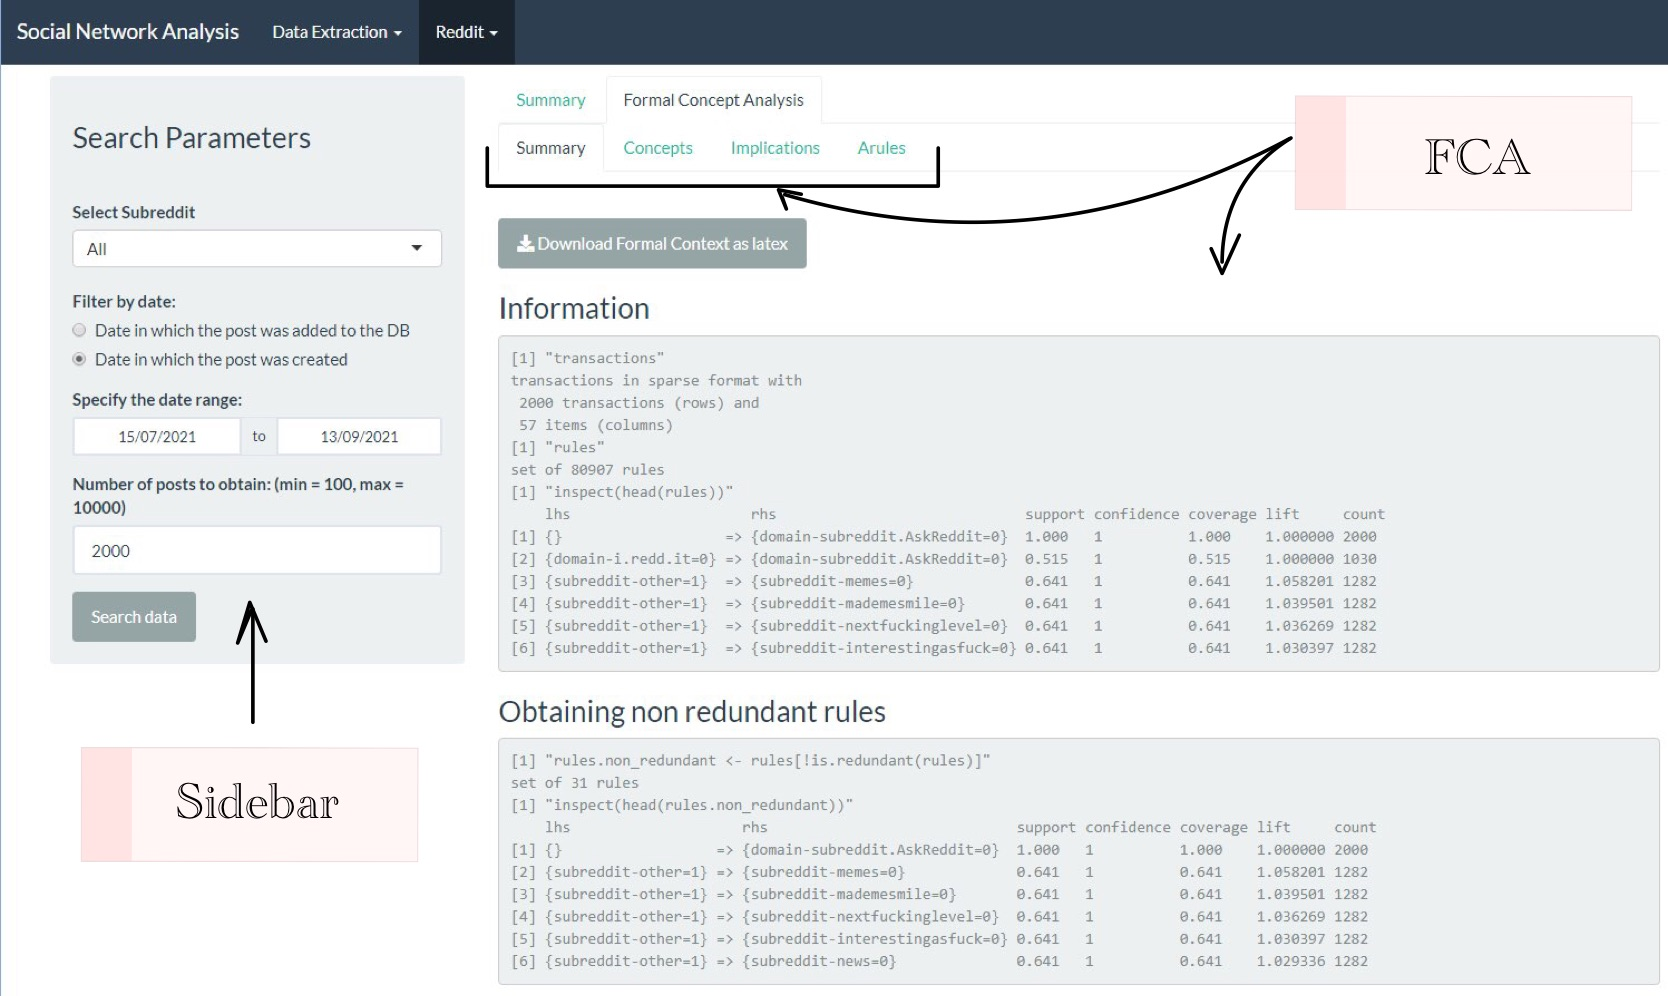
\includegraphics[width=400pt]{images/implementacion/app-4.jpg}
\caption{Aplicación \Gls{shiny} - Módulos en Análisis de Conceptos Formales}
\end{figure}
        

\end{document}